\chapter{Architecture}
\label{chap:architecture}

The following section will define the data model each peer keeps of its data and specify the API for updating it between peers, both trusted and encrypted.
Therefore we start this chapter with an explanation of all meta information that a trusted peer stores, as everything else is based on top of this information.
Then we will define and explain the model each peer keeps of the stored data.
Built on this model we will discuss the messages used to facilitate the update of the model between clients.
Then we will discuss the protocol extensions required for the encrypted model.
Finally we will take a look at the advanced features and how they can be built on top of the previous work.

We chose to use JSON for all communication between peers as further discussed in section~\ref{sub:JSON}.
Therefore generally speaking all messages will be defined as JSON messages.
Additionally most data is written to storage as JSON files.
This has the advantage of allowing easy manual access to all files and message for development purposes since JSON messages can be sent as simple text messages via the normal Tox chat clients.

\section{Meta Data}
\label{sec:Meta Data}

Since a trusted peer must store the last known state of the directory to detect changes for later synchronizations, we must store this information to storage somewhere.
For Tinzenite we took a page from Git and decided to write this information within the directory to be synchronized.
To reduce visual clutter and to hide it from users this directory is offered by a hidden directory directly below the root directory.
We specified it as \textit{".tinzenite"}.
In short it contains organizational files, temporary objects, and the deletion directory for storing files until they have been fully removed by all peers, plus data private to the peer.
Figure~\ref{list:meta_folder} gives a broad overview of the contents.

\begin{figure}[htp]
\begin{modellist}
\item .tinzenite/
\begin{modellist}
    \item org/
    \begin{modellist}
        \item peers/
        \item auth.json
    \end{modellist}
    \item removed/
    \item temp/
    \item receiving/
    \item sending/
    \item local/
    \begin{modellist}
        \item rmstore/
        \item model.json
        \item self.json
    \end{modellist}
    \item .tinignore
\end{modellist}
\end{modellist}
\caption[Meta Folder Structure]{Overview of the special meta information directory that Tinzenite uses to store relevant information required for the managing of the directory. For brevity sub directories that contain instance data are not expanded.}
\label{list:meta_folder}
\end{figure}

Placing the meta data within the directory has a few benefits for the complexity of the system and enables it to utilize the full feature set of the implemented synchronization capabilities to share data between peers when required.
Specifically only the \textit{"org"} directory and the \textit{"removed"} directory are synchronized just as any user data, along with the \textit{".tinignore"} file which specifies to ignore all other objects in the meta directory.
The choice to use Tinzenite itself to handle these directories and files was done as they are required for trusted peers to work correctly.
The \textit{"org"} directory is included because it contains both the authentication file and the peer files -- both are required to be kept synchronized between all other trusted peers.
The \textit{"removed"} directory is included due to how removals must be handled as discussed in section~\ref{subs:Remove}.

\subsection{Organizational Directory}
\label{sub:Organizational Directory}

The \textit{"org"} directory consists of two objects: the file containing the authentication information and a sub folder which contains a file for each known peer.
It is first of two directories that are synchronized along with user specified files between peers, as both the authentication file and the peer list are required for all peers to function correctly.

\subsubsection{Authentication File}
\label{subs:Authentication File}

The authentication file stores information required for the complete Tinzenite network.
This includes information on the user, information on the directory the network synchronizes, and the encryption keys required to encrypt and decrypt data for encrypted peers.
Since the authentication file is not encrypted upon upload to encrypted peers as it is meant to be used to enable user account management, all personal or otherwise critical information is stored either hashed or fully encrypted.
Listing~\ref{json:auth_object} shows the contents of an example authentication file.

\begin{listing}[htp]
    \begin{lstlisting}[language=json,firstnumber=0]
{
    "User": "$2a$10$E8Wlr9Jn/EYJLZ7J0yZoR.Qscp.MKD2kG8dHF7OQWYNA1mCfp.Qqe",
    "Dirname": "sync",
    "DirID": "ffff1d4cbfded232",
    "Secure": "Kbk4+sx17VKHma1Z67OU6R7TbHPWMr4SpZhWUQqheS/CNcKKHVYjTTSv0rbF4qDAa0vwikigsm7wHhy4iGjWB84i0ErO7rNwhqrPPxudeDM=",
    "Nonce": [255,142,165,173,201,188,98,116,29,31,173,181,84,84,137,54,159,50,193,248,51,162,76,195]
}
    \end{lstlisting}
\caption[Authentication JSON Object]{An example of an authentication file.}
\label{json:auth_object}
\end{listing}

The key \textit{"User"} stores a bcrypt hash~\cite{provos1999future} of the user's name.
This is important for example for the support of encrypted third party peers: they can attach accounts to the provided user name for controlling server side access.
It provides a way to enable encrypted server service providers to attach their own accounts directly into a Tinzenite network so that access can be managed.
The user given name of the directory is stored in \textit{"Dirname"}.
It is not hashed so that the user can easily read which directory the current authentication file belongs to.
We also need a way to distinguish multiple synchronized directories from each other: this is the random unique hash stored in \textit{"DirID"}.
This unique identification also allows us to differentiate multiple Tinzenite networks that might share a directory name.
Again, this can be used by third party service providers to differentiate the amount of directories that a user can store with them.
The encryption keys for encrypting and decrypting file data for encrypted peers is stored in \textit{"Secure"}.
These keys are encrypted with a password derived encryption scheme further discussed in section~\ref{sub:Key Encryption}.
\textit{"Nonce"} stores the nonce value that is required additionally to the user provided password to successfully access the encryption keys.

\subsubsection{Peer Files}
\label{subs:Peer Files}

Within the \textit{"peers"} folder Tinzenite writes all data related to synchronization peers.
It is in essence the contact list, filled with information required to access peers.
This includes a peer's address, trust, and further user defined information.

\begin{listing}[htp]
    \begin{lstlisting}[language=json,firstnumber=0]
{
    "Name": "box",
    "Address": "b6ad2388839d3068f9d6562c10d1151dd87818373c88cf9aad829144c63aac36",
    "Protocol": 1,
    "Trusted": false,
    "Identification": "19baf5873da66797"
}
    \end{lstlisting}
\caption[Peer JSON Object]{An example of a peer JSON object. Note that the encryption attribute is not to be trusted, it is only an optimization.}
\label{json:peer_object}
\end{listing}

Listing~\ref{json:peer_object} shows the structure of an example peer file.
One of these must exist for all known peers.
The \textit{"Name"} is the user defined name for each peer, to be used by the user to make differentiating between peers easier.
Internally however the peer is referenced by the random assigned hash stored in \textit{"Identification"}.
The Tox address is stored in \textit{"Address"}.
Whenever a new peer is added and its peer file distributed to all known peers, they can use this information to automatically accept connections to the new peer.
The \textit{"Trusted"} attribute is an optimization: peers for which this value is false don't need to receive and decline a challenge.
It is important to note that the other way around is not true: if the value is false the other peer must still respond successfully to a challenge.
Finally the \textit{"Protocol"} value defines via which protocol the peer can be reached.
This is currently unused as we only use Tox.

\subsection{Removed Directory}
\label{sub:Removed Directory}

\begin{figure}[htp]
\begin{modellist}
\item removed/
\begin{modellist}
    \item db198086d1708794/
    \begin{modellist}
        \item check/
        \begin{modellist}
            \item 927325d7a930dac9
            \item ec021135799691ae
        \end{modellist}
        \item done/
        \begin{modellist}
            \item 927325d7a930dac9
        \end{modellist}
    \end{modellist}
\end{modellist}
\end{modellist}
\caption[Removed Folder Structure]{Example of the removed directory with an active removal pending. Note the missing file in \textit{"done"} which would signify the completion of the removal.}
\label{list:removed_folder}
\end{figure}

The \textit{"removed"} directory stores objects that are pending removal as described in section~\ref{subs:Remove}.
An example of the directory with a pending removal can be seen in figure~\ref{list:removed_folder}.
Notably this directory is synchronized among Tinzenite peers just as any data the user synchronizes.
This is due to the fact that removals must be synchronized by all peers.

For each object that is removed a directory with the object's identification is created.
Within this directory two sub directories are created in which empty files named after peer identifications are placed.
In the \textit{"check"} directory peers write a file named after each peer who must confirm the removal.
The \textit{"done"} directory contains a file named after every peer that has applied the removal and is now also waiting for it to complete.

\subsection{Unsynchronized Directories}
\label{sub:Unsynchronized Directories}

All other directories within the \textit{".tinzenite"} directory are not synchronized between peers as they are only used to store locally relevant data.
The file which contains the rules for this is the \textit{".tinignore"} file (for more information on ignore rules see section~\ref{subs:Ignoring Objects}).

The \textit{"temp"}, \textit{"received"}, and \textit{"sending"} directories are used for files in transit either in preparation before being sent encrypted or upon receiving before being applied to the local directory.
Files are transmitted by chunks by Tox.
Therefore, to keep the RAM storage requirements down, these blocks are immediately written to storage.
This also avoids partially overwritting user accessible files if the transfer fails for some reason, thus ensuring that Tinzenite only overwrites the user's files when it is ready to do so with a complete file.

The \textit{"local"} directory is used for three purposes.
First a copy of the peer's own peer information is written into a file alongside with a binary dump that the underlying Tox channel requires to run which contains the persistent state information.
Second the actual model is written to storage here, although not as a fully expanded object tree as specified in section~\ref{sec:Object Model}.
Instead Tinzenite writes the internal representation of the model to storage as JSON.
This differentiates in a few key points, but primarily serves to store both the absolute path and to keep the directory tree in a flat representation that is more efficient to actually work with.
Finally the \textit{"rmstore"} directory keeps a record of all previously completed removals in the case that a peer tries to reintroduce a completed removal.

\section{Object Model}
\label{sec:Object Model}

This section will describe our solution to how Tinzenite keeps track of objects within a directory.
This data will be henceforth referenced to as the data model or just model.
Based on this we will highlight how Tinzenite applies object operations on the model in a further section.

The model is required to enable detection of newly created and removed files, since Tinzenite does not actively watch a directory.
Having a stored representation of a directory significantly eases the difficulty of detecting file creations and removals, even if the peer software is not running.
Any entry in the model is generally referred to as an object if the distinction between a directory or file is not required.

An important feature that the model should have is that it should represent an arbitrarily complex object structure in the most simple way possible.
Therefore there are only two assumptions we will make for the structure of any directory: namely that it contains files sorted in nested directories.
Out of this tree view we can immediately synthesize our two main components that we will require: a file model (a leaf) and a directory model (a node).
Since a peer is intended to have a directory as the root node from which to run, the core element will always be a directory.
An example of the proposed model structure can be seen in~\ref{list:model}.

\begin{figure}[htp]
\begin{modellist}
\item Root Directory/
    \begin{modellist}
        \item .tinzenite/
        \item Sub Directory/
            \begin{modellist}
                \item File
                \item File
            \end{modellist}
        \item File
        \item File
    \end{modellist}
\end{modellist}
\caption[Data Model Example Structure]{An example of how a data model of a directory is structured. The .tinzenite directory is discussed in section~\ref{sec:Meta Data}.}
\label{list:model}
\end{figure}

Since each file is considered a binary blob and must not be modified by Tinzenite in any way to preserve data integrity, any additional information that Tinzenite is required to store for an object must be kept within the model itself.
Out of this we can see which values need to be stored within the model for each object specifically.

Each object in the model will be specified for identification purposes by a unique randomly generated hash.
This hash allows us to decouple the name of the object from its model representation, effectively serving as the same function as node identification numbers when stored on a hard drive.
Furthermore each model object will contain a path variable that specifies the relative path of the object in the directory tree.
This has the purpose of allowing the placement of all files in the correct locations on storage for a given root path.

\begin{listing}[htp]
    \begin{lstlisting}[language=json,firstnumber=0]
"Version": {
    "927325d7a930dac9": 1,
    "19baf5873da66797": 4,
    "ec021135799691ae": 3
}
    \end{lstlisting}
\caption[Version JSON]{An example of a version vector clock. Each hash is the identification of a trusted peer, the associated number which version of an object they last modified.}
\label{json:version_model}
\end{listing}

Apart from the above attributes Tinzenite must also track versions of files to allow detection of when objects have been updated.
We will use a vector clock~\cite{mattern1989virtual} to implement this, where entries represent peers and the associated number is the last version where that peer actively contributed to the object's history.
The vector clock can also be used to detect collisions.
Note that the vector clock must only store the versions for active, trusted peers as these are the only peers where versions can differ upon user interaction.
We avoid using a simple dirty flag for reasons of complexity: determining which peer's update to take in which order is not trivially doable with a simple boolean flag.
Utilizing vector clocks gives us greater flexibility, both for the implementation and for any visualizations in the case of tracing changes.
An example of the vector clock as we will use it can be seen in listing~\ref{json:version_model}.

It is important to note that the model will not be used to store peer reliant information.
This includes for example where the directory is placed on the peer's file system, which may differ between peers.
Such information must be stored separately by the peer and be applied when working with the data model, for example when determining what the full path on the file system will be for a file that is to be written.
Some properties are also not suited to be transferred between peers.
This includes file system or operating system dependent properties such as usage rights, ownership, or flags.
For Tinzenite we will generally ignore these as the primary focus is just raw data synchronization without semantic information.

\subsection{Directory Model}
\label{sec:dir_model}

\begin{listing}[htp]
    \begin{lstlisting}[language=json,firstnumber=0]
{
    "Directory":true,
    "Identification":"db198086d1708794",
    "Name":"test",
    "Path":"test/test",
    "Shadow":false,
    "Version":{},
    "Objects":[]
}
    \end{lstlisting}
\caption[Directory JSON Model]{An example of a directory JSON object. Note that for brevity no files or sub directories are shown in the \textit{"objects"} array. The version object is also left empty here.}
\label{json:directory_model}
\end{listing}

Listing~\ref{json:directory_model} shows an example of the proposed JSON structure for representing a directory.
A directory is somewhat special as it does not require the synchronization of an attached binary file.
This is the case for Tinzenite because directories are viewed independent from their content.

The \textit{"identification"} attribute is a random generated hash that uniquely identifies the directory.
The \textit{"path"} attribute stores the concatenated relative full path from the peers root directory to where the directory lies.
The clear text \textit{"name"} is also stored here as an attribute.
The \textit{"shadow"} flag is used to signal whether the contents of the directory are to be fetched or not.
To differentiate between updates we require a \textit{"version"} attribute which represents a vector clock of peers and their last known version.

Finally an \textit{"objects"} array is where the corresponding sub directories or files are recursively placed.
To model a directory as shown for example in figure~\ref{list:model} Tinzenite begins the model with a directory model for the root directory.
Within the objects array one can the then find the two files and the two further directories.
Each directory object in turn also stores sub objects in its object array, thus recursively modeling an entire directory.

\subsection{File Model}
\label{sec:file_model}

\begin{listing}[htp]
    \begin{lstlisting}[language=json,firstnumber=0]
{
    "Directory":false,
    "Identification":"b83cf06d4e056e1a",
    "Name":"else.txt",
    "Path":"test/else.txt",
    "Shadow":false,
    "Version":
    {
        "927325d7a930dac9":1
    },
    "Content":"e4abda92f30700d751ac82f7454787d5"
}
    \end{lstlisting}
\caption[File JSON Model]{An example of a file JSON object.}
\label{json:file_model}
\end{listing}

Listing~\ref{json:file_model} shows an example of the proposed JSON structure for representing a file object.
The \textit{"identification"} attribute is a random generated hash that uniquely identifies the file.
The \textit{"path"} attribute stores the concatenated relative full path from the peers root directory.
The clear text \textit{"name"} is also stored here as an attribute.
To differentiate between updates we require a \textit{"version"} attribute which represents a vector clock of peers and their last known version of this file.
Important for detecting file changes is the \textit{"content"} attribute which stores a hash of the file's binary blob.
Finally the \textit{"shadow"} flag is used to notify a peer whether the file is locally accessible or must first be fetched from other peers.

\subsection{Object Operations}
\label{sub:Object Operations}

Based on the defined model we will now discuss which file or directory operations are applied in what way to the model.
Tinzenite relies only on the most basic file operations for manipulating both the model and the actual file directory.
Therefore we require only the following four operations for the basic case to work:

\begin{description}[leftmargin=5em,style=nextline,noitemsep,nolistsep]
    \item[Create]
        Created files are detected by simply noticing files that do not exist in the model yet and are not listed as removed.
        Files that have been created will be added to the model at the correct location and their attributes calculated, if not given.
        Tinzenite then checks whether it needs to fetch the file if it wasn't created in its own directory instance.
    \item[Modify]
        Modification is either when the model does not match the file anymore, in which case a new file must be fetched, or the content of the local file has changed.
        This is detected via the content hash\footnote{Since hashing a file is an expensive operation we have also implemented that the hash is only checked if the modtime of the file has changed since its last update. This greatly speeds up checking for modified files.}.
        The model is updated to match the file again.
    \item[Remove]
        A removal is detected when a file does not exist anymore and was previously tracked by the model.
        File removing is one of the most complex cases in Tinzenite due to the insert delete ambiguity.
        We will solve this by storing the models of deleted files until the delete update has been propagated to all currently known peers.
        Only then the model is also discarded.
        For this to work Tinzenite must always ensure that files that exist but are listed as deleted are not added back to the model as a new file by continuously checking the deletion list.
\end{description}

These three operations are not the only operations that a user can do on directories or files.
However they are all the operations that Tinzenite requires so that it can cover all possible file state transitions.
The choice of these three basic operations for Tinzenite was heavily based on the paper discussed in section~\ref{sub:An Algebraic Approach to File Synchronization}.

\begin{figure}[tp]
\centering
    \includegraphics[width=4cm]{graph/sm_object_lifecycle}
\caption[Object State Diagram]{The life cycle of every object, file and directory, in Tinzenite with the allowed operations.}
\label{diagram:object_operations}
\end{figure}

Therefore the life cycle of an object is very simple, as can be seen in figure~\ref{diagram:object_operations}.
Objects can only come into existence via the create operation.
Objects can either be changed by changing their content which is a modify operation, or by changing their location which is a move operation.
Finally objects can also be removed.
If an object has been removed it will stay removed unless the user creates a new clone of it.

In the following sub sections we show the actual definition of the specification and expand on how Tinzenite peers react to them in more detail.
This specification makes up the core functionality of how the data synchronization happens within Tinzenite.
Note that these operations are only for trusted peers: since encrypted peers can not work on the stored data they have no need for the file operations.

\subsubsection{Create}
\label{subs:Create}

The creation of an object can be trivially detected in Tinzenite.
Basically there are two cases where an object must be created: the first is local manual creation which implies that the peer is the origin of the file; the second is creation via receiving a creation message from another peer.

In the first case, if the object does not have a representation within the model and is not listed as removed, it triggers the creation case.
Tinzenite creates the correct object representation and inserts it into the correct place in the model.
This includes creating the unique identification hash and, if the object is a file, creating a hash of the file contents.
For a remote creation the peer will queue a fetch operation for the required file.
Only when the file has been received completely it is placed at the correct location and the model will be updated.

\subsubsection{Modify}
\label{subs:Modify}

The modification of an object is not as trivially detected as an object creation.
Special care must be taken in the case of conflicting changes which can obviously happen since the directory is shared among multiple peers (see section~\ref{sec:Update Detection and Reconciliation}).
Here we will only consider what happens once a modification has been detected.
Again we have two possibilities for triggering this case: a local file has been modified or the peer has received an update message for a remote modification.

If the modification is detected locally we update the model to match the new directory state for that object and then initiate an update message.
If, on the other hand, we receive a remote modification, we queue the fetching of the updated file.
Upon receiving the changes we apply them and finally propagate the update to the other connected trusted peers.

\subsubsection{Remove}
\label{subs:Remove}

Finally the deletion of an object is the hardest case within Tinzenite because of the insert delete ambiguity as discussed in section~\ref{sub:Perspectives on Optimistically Replicated, Peer-to-Peer Filing}.
It is nontrivial to ensure that an object deletion has been received by all required peers so that it truly and finally can be removed from the complete Tinzenite network.
A simple solution would be a list of all deleted objects ever, but this list would promise to grow quickly on often used synchronized directories.
Therefore we require a sort of garbage collection so that we can trim the list from deleted files that have been applied to all known peers.

We will look at Tinzenite's deletion of an object that has been removed locally first, then discuss how the update propagates and what the other peers are required to do to ensure a safe and complete deletion.
Upon detection of a local deletion the trusted peer creates a directory within the \textit{"removed"} directory with the name of the removed object's identification hash.
Within this directory the peer copies the list of currently known trusted peers\footnote{Note that encrypted peers must not be considered because they basically mirror only active peers, meaning they are guaranteed to correctly apply deletions once the active peers have reconciled it.} to the \textit{"check"} sub directory.
We utilize simple empty files named after the peer identification hashes as entries since that is all the information we require for a deletion.
We will refer to these files as the peer entry files for the purpose of describing the rest of the operation.
To complete the removal operations required to initiate the removal through the Tinzenite network, the peer writes another peer entry file to the \textit{"done"} sub directory.
This sub directory contains a peer entry file for all the trusted peers that have acknowledged receiving the deletion update.
For an example of a removal directory for a file, see figure~\ref{list:removed_folder}.

Since the removal directory is also synchronized to all trusted peers they can continue applying the removal.
Each peer receives first the creation of the removal directory and the deletion message for the object.
Once the removal has been locally applied each peer writes a peer entry file to the \textit{"done"} directory -- so long as it finds a corresponding file in the \textit{"check"} directory.
If the peer knows of peers that do not have a peer entry file in the \textit{"check"} directory it must append them.
This guarantees that all peers that have known of the existence of an object will receive its removal.
An example of where this appending is vitally important is when a new peer has recently been added to the Tinzenite network but its creation has not yet reached the deleting peer.
In this case at some point the removal and the creation of the new peer will collide and the peer where the collision happens will append the newly created peer to the \textit{"check"} directory.
This guarantees that even though the peer where the removal originated from did not know of all peers, it will still wait for the new peer to also apply the removal.
This is guaranteed to happen as the new peer entry file for the appended peer will reach the peer where the removal originated from before the removal is completed in any case.

Once the last peer enters itself into the \textit{"done"} directory it propagates the update one final time and can then deletes the removal directory.
It is important to note that this deletion differs from other tracked removals: unlike when any other object is removed, deletions within the \textit{"removed"} directory must not trigger another round of tracked removals.
This would cause an endless removal of removals and basically bring the entire Tinzenite network to a halt as each peer is swamped with keeping up.
Instead the objects and associated model entries are simply silently purged.
Yet since it is very likely that not all peers delete the removal directory at the same time we must guard it against being unnecessarily reintroduced.
Therefore each peer must locally remember each deletion for a specified time span until it can be sure that all peers have applied the completed deletion.
During this time span each peer ignores the reintroduction of the deleted objects\footnote{As an improvement to this behavior we also utilize notification messages to more rapidly terminate removals. See section~\ref{subs:Notify Message} for more details on this.}.

Now a final note on what happens should a peer receive a deletion update for an object that it doesn't know.
In this case the message can not simply be discarded silently as there is no other representation of the update in the object model.
This could lead to orphaned updates if the peer acts as a bridge between two peers that were previously directly connected.
Therefore unknown deletion updates should be propagated if possible.
However, since orphaned updates can only happen as long as the peer list has not been fully updated between all peers, this is a sufficiently unlikely case that we can live with.
By adding a time stamp we can even detect orphaned deletion updates and warn the user to help solve the issue.
Alternatively we can also warn if we have too many possibly orphaned updates, although this would signify a larger issue.
Since there is no way to reliably ensure that all peers are in the same state simply for the reason that a peer may be offline at any point, there is little more we can do to ensure clean removals.
%NOTE: this is a good philosophy for Tinzenite, remember it for presentation! :D
It is more important to work towards a common model state than to ensure that previous states were legitimate for all peers.

\section{Communication Specification}
\label{sec:Communication Specification}

This section describes the specifications for the messages that will be used to synchronize two models on separate peers.
We start with defining how connections are managed, then build on this to explain how new peers are added to an existing network.
Then we will specify the messages used for model synchronizations between trusted and between trusted and encrypted peers.
Finally we will briefly expand on the ordering of messages and the expected emerging behavior.

Every peer views all connected peers as separate connections.
A swarm behavior only comes to pass because of the independent actions of every peer, not through a combined communication between multiple peers.
This primarily makes it relatively easy to implement a Tinzenite peer, as the communication state is never between multiple peers.
Therefore a single peer has a base state of no other connected peers.

\subsection{Connection Management}
\label{sec:conn_management}

In this section we will discuss how Tinzenite connects to other peers.
As we distinguish between trusted and encrypted peers we must determine how the data we will send is to be modified accordingly.
Note that encrypted peers by default will not initiate connections, only trusted peers will do that as they are the only peers capable of working on the user's data.
Encrypted peers in general have a very passive role in the Tinzenite network.

Since each trusted peer has access to a list of all connected peers (see section~\ref{sub:Organizational Directory}) this list is used for the initial presumption which connected peer is trusted and which is encrypted.
Therefore peers marked as encrypted are not even issued a challenge to authenticate themselves.
To vet trusted peers however the challenge must be issued and met.
Consequently the trusted peer queries each trusted connected peer in turn.
Since we should not trust a peer just because it has been marked as trusted, this query must be cryptographically secure.
An attacker that wants to connect to a trusted peer illegitimately thus can not establish a clear connection without the required keys, which the attacker should not be in possession of\footnote{Tinzenite is designed to avoid revealing keys to outsiders. However attacks such as key loggers are beyond its control.}.
We define this as the authentication challenge.
Only if the challenge is successfully answered the other peer is considered trusted and the following communication will not be encrypted.
If the challenge is answered incorrectly or not at all we can not be assured that the other peer is either trusted or encrypted.
Therefore we simply ignore it for all further operations\footnote{Ideally we would warn the user of this as it may result in peers being orphaned within the network. Since this requires either the user having tried to connect to an insecure peer or a peer having become compromised, the chance that this behavior is undesired is comparatively small.}.
This concludes opening a communication channel with a connected peer.

\begin{figure}[tp]
\centering
    \includegraphics[width=6cm]{graph/sm_peer_communications}
\caption[Connection State Diagram]{This diagram shows how peers handle the establishment of a connection to a known peer.}
\label{graph:connection_states}
\end{figure}

Figure~\ref{graph:connection_states} shows an informal state diagram of how a peer reaches the idle state where the connection is ready and set up, both for trusted and encrypted peers.
The switch from the disconnected state to the connected state is signaled by the underlying Tox connection, meaning it happens when the other peer is online and visible via the Tox channel.
Once connected and if the peer itself is a trusted peer, a challenge is sent which contains an encrypted nonce.
For a more comprehensive look at the challenge response mechanism see section~\ref{sub:Challenge Response}.

Note that a few points must be considered that can not be shown in the diagram.
Since Tinzenite is designed as a peer to peer network, no client-server structure exists.
This poses the challenge of who begins the construction of a connection, especially as we can not distinguish between peers that have been online for a while already and peers that just become activated when the base peer connects to the network.
This is due to peer to peer architecture of Tox: not all peers will respond to queries within the same time frame.
From a network perspective peers that are further away will seem to be online slower than peers that are nearer.
We solve this issue by having the peers use a random back off time whenever a request expects an answer\footnote{For example the challenge message for establishing a trusted connection.}.

Since we can not trust the other side of the Tox channel to be a Tinzenite peer, the peer initiating a connection will not advance beyond the step where it expects an answer.
This means that for example an attacker would either receive only a challenge (to which he can't respond without knowing the keys) or the request for the meta information block to which he'd have to answer correctly.

A short note on closing a connection: once established this happens when the underlying Tox channel is terminated.
Furthermore if something interrupts the establishment of a connection, both peers will simply go back to the starting point.
Establishing a connection is done every time a peer reconnects.

\subsection{New Connection Establishment}
\label{sub:New Connection Establishment}

The previous section described how Tinzenite connects to known peers.
This section therefore discusses how Tinzenite connects to new peers, meaning peers that the user adds to the network.
Notably this is a manual process where the user is used as a secondary channel to prevent man-in-the-middle attacks.
Since a typical Tinzenite network might have many peers, it is not desirable to have to authenticate a new peer manually with every other peer.
We therefore propose that the user only needs to authenticate the new peer with one existing trusted peer.
From there the authentication is synchronized to the other existing peers much like any other file or property update.
This bootstrapping process allows a user-friendly setup of peers.

\begin{figure}[tp]
\centering
    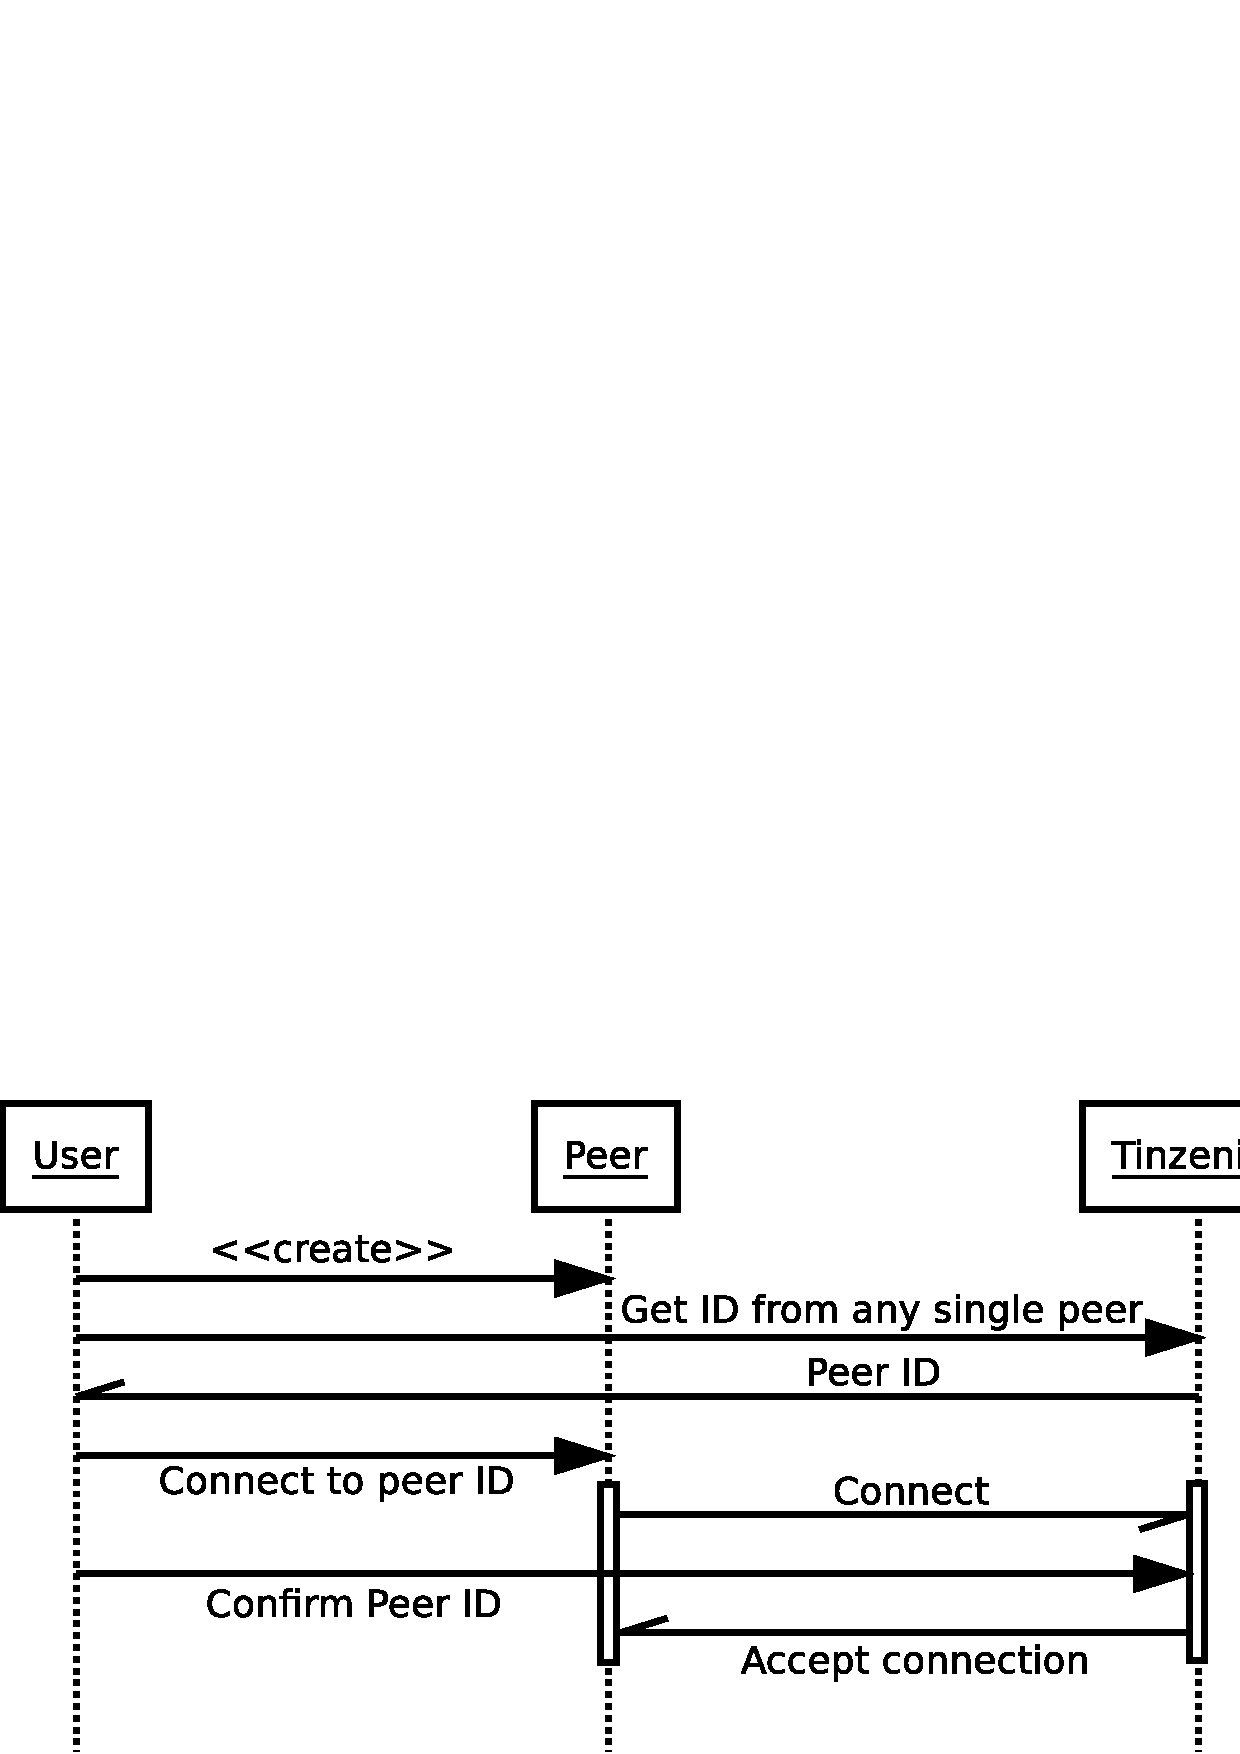
\includegraphics[width=10cm]{diagram/sequence_new_connect}
\caption[New Connection Sequence Diagram]{This diagram shows the interaction required to connect a new peer to the existing Tinzenite network.}
\label{diagram:new_connection}
\end{figure}

Figure~\ref{diagram:new_connection} shows how a user interacts with a Tinzenite peer and the Tinzenite network (consisting of 1 to n other existing peers) to connect a new peer to the network for the first time.
As prose: the users simply start the new peer client for the first time, whether encrypted or trusted.
Then they can point it at the directory location, change settings, and check whether a trusted peer is available.
To establish an initial connection a Tox ID of an available Tinzenite peer is required.
The users can then command the new peer to connect to this available peer by entering the Tox ID.
To ensure that no man-in-the-middle attack can happen the users will now have to confirm to the connection the available peer.
This means allowing the connection there and ideally ensuring that the seen Tox ID is identical with the new peer's Tox ID.
Tinzenite then reports to the user whether the newly connected peer requested can be registered as a trusted peer or not.
Once the connection has been confirmed for the given trust level on the other peer the channel is opened and ready.

What happens next differs somewhat depending on whether the new peer is an encrypted or a trusted peer.
Since encrypted peers are passive peers the bootstrapping process is finished once the peer has established a connection to a trusted peer.
However the encrypted peer at this state still lacks any encrypted files or more importantly the list of other peers and the authentication file.
It falls upon the connected trusted peer to initiate the first data upload, after which the new encrypted peer will have all the required information.

If the new peer is a trusted peer it must autonomously complete the bootstrapping by fetching all the files from the existing peer.
This works even without an authentication file because the existing peer has received user confirmation of the trust status of the bootstrapping peer.
This allows it to fetch all files unencrypted.
Once all files have been fetched the new trusted peer is ready to run.
This includes immediately connecting to other existing peers since the peer list is now also available to it.

Even if the new peer goes offline immediately after completing the bootstrap process, the new peer information will be synchronized throughout the already connected peers once they synchronize with the peer which accepted the new peer.
This is possible because the connection request by a new peer includes its own peer information, and when the connection is accepted this peer information is immediately added to the \textit{"peers"} directory.
Thus it will be synchronized to all other peers who will automatically accept any connections of peers listed in the peer list.

Removing peers will work much in the same way from a system perspective.
A user can note a peer to be removed, resulting in it being removed immediately from the peer where the action was initiated.
The removal will then transit through online peers and result in a complete removal once all peers have been online.
An interesting aspect to how to handle removal from the perspective of the removed peer is what to do with the remaining data.
For a trusted peer we might offer a choice whether to remove the data or simply disconnect it from the Tinzenite network.
On the other hand encrypted peers can simply remove the data immediately as they can't access it anyway.
Notably removing a peer requires no action on the removed peer's side.
This ensures that a peer can be excluded even if direct access to the peer was lost.

\subsection{Message Order}
\label{sub:Message Order}

We must define which messages are required to be sent when to keep two models between peers synchronized.
Once the connection is established we must differentiate between trusted peers and encrypted peers.
For trusted peers a connection is only considered established after the \nameref{subs:Authentication Message}s have been exchanged.

For trusted peers we propose the following message timing to enable rapid propagation of updates throughout the network.
Upon connection both peers will first exchange models, providing essentially a snapshot of differences since the last synchronization.
This requires a message to request the model from the other peer.
Since we will also need to request files we use a generalized \nameref{subs:Request Message} that can trigger a file transfer.
Upon reception of the model, both peers will merge the models and request any changed files.
At the end of a model request both peers should share a common model state and associated directory state.

If local changes happen during or after the model has been exchanged the \nameref{subs:Update Message}s are used to notify the other model of the update without having to retransmit the entire model again.
However to ensure that all updates do propagate at some point, ideally rather faster than longer, we propose that each peer resends the model every few units.
The exact spacing of when the complete model is resent is again up to the peer itself and can be adjusted per instance.
This allows mobile peers to work more energy efficient by synchronizing less often in comparison to desktop peers where power and bandwidth usage don't play such prominent roles.

Since encrypted peers work passively it is again up to the trusted peers to ensure that they are queried regularly.
To avoid creating merge conflicts on encrypted peers which these could not independently resolve since all data is encrypted, encrypted peers can only be accessed by a single trusted peer at the same time.
This will be negotiated via \nameref{subs:Lock Message}s.
Once successfully locked request messages can be used to fetch data from the encrypted peer.
To place data on the encrypted peer we thus require a \nameref{subs:Push Message}.

\subsection{Trusted Synchronization}
\label{sub:Trusted Synchronization}

Now that we have discussed how a peer is structured and how its connections are handled, we can turn to how a trusted peer receives and sends messages via the Tox channel.
Once the setup has been completed, as seen in section~\ref{sec:conn_management}, the models must be updated if they do not match.
This happens normally when files and directories have changed through user interaction.

\subsubsection{Authentication Message}
\label{subs:Authentication Message}

The authentication message is used to verify trusted peers against each other to ensure that clear text data is only sent between themselves.
The same method is used for both challenge and response.
For a more in depth look into how the mechanism works see section~\ref{sub:Challenge Response}.

\begin{listing}[htp]
    \begin{lstlisting}[language=json,firstnumber=0]
{
    "Type":"challenge",
    "Encrypted":"5HFXCQBMwe6ohx9fKeLsNxaBsOK7+9pxWFiXX4aE4cRtdt8oUOHQBJ6XrowiwwgLunM="
}
    \end{lstlisting}
\caption[Authentication Message]{An example of a valid authentication message containing a challenge.}
\label{json:authentication_message}
\end{listing}

Listing~\ref{json:authentication_message} shows an example of a challenging authentication message.
The \textit{"Encrypted"} value contains the challenge value or the response value encrypted with the data encryption keys.

\subsubsection{Request Message}
\label{subs:Request Message}

In general each peer does not rely on other peers to update.
Therefore we propose the creation of request operation which serves to request resources required for synchronization with another peer.
This request can be used both for the complete directory model as for each specific file.
It is important to note here that directories should never be requested as they do not require attached binary data to be either created, modified, or removed.
Thus a request operation is only for operations that require data to be transferred.
Upon receiving the message the other peer starts a Tox file transfer which the initiating peer knows to accept as it just requested it.

\begin{listing}[htp]
    \begin{lstlisting}[language=json,firstnumber=0]
{
    "Type":"request",
    "ObjType":"object",
    "Identification":"b83cf06d4e056e1a"
}
    \end{lstlisting}
\caption[Request Message]{Example of a JSON request message.}
\label{json:request_message}
\end{listing}

Listing~\ref{json:request_message} shows how a message to initiate a file transfer is structured.
\textit{"ObjType"} can have the values object, peer, model, or auth.
The peer and auth values are used by the encrypted peer to differentiate these special meta data from normal encrypted files.
\textit{"Identification"} is the unique hash that each object is referenced by.

By switching the \textit{"ObjType"} attribute from object to model the other peer, whether encrypted or trusted, can be commanded to send its current model.
After comparing the received model to its own model, the peer knows for which files it must request data.
Thus actively requesting a full model update periodically will still allow updates to propagate independent of individual update messages at some point in time.

This message is also explicitly used to get an encrypted peer to initiate a file transfer of the requested file or the encrypted model.
The encrypted peer will respond with a file transfer of the requested object if the trusted peer has successfully locked it.
If not, the trusted peer will receive lock denial messages until it has successfully locked the connection.

\subsubsection{Update Message}
\label{subs:Update Message}

Continuously requesting and receiving the model is not ideal.
For large directories just the transfer of the model may require significant bandwidth.
Therefore we have included the option of sending current updates to all currently connected trusted peers so that they can apply the update without first having to request the complete model.

\begin{listing}[htp]
    \begin{lstlisting}[language=json,firstnumber=0]
{
    "Type":"update",
    "Operation":"modify",
    "Object":
    {
        "Directory":false,
        "Identification":"b83cf06d4e056e1a",
        "Name":"else.txt",
        "Path":"else.txt",
        "Shadow":false,
        "Version":
        {
            "927325d7a930dac9":3
        },
        "Content":"cecef410a6ef0d3c3e101ab726af2776"
    }
}
    \end{lstlisting}
\caption[Update Object Message]{The message broadcast by a peer to connected peers to notify that an update has happened.}
\label{json:update_object}
\end{listing}

Listing~\ref{json:update_object} is a message for broadcasting a model update to other connected trusted peers.
\textit{"Operation"} can be any value of either create, remove, or modify.
The key \textit{"Object"} contains the object representation for the updated object as seen in section~\ref{sec:Object Model}.

The update message serves to keep both models in sync even after the initial synchronization at connection establishment.
Upon receiving an update message the peer should immediately respond with a request message to retrieve the updated file.
If a peer receives a message for an operation that it has already applied, the message is silently discarded.
This does not disturb the propagation of updates since the peer will have sent the update to the other connected peers if it  already has the update.
In this way we ensure that every message propagates as far as possible without consuming unnecessary bandwidth\footnote{Peers are of course free to implement message sending in any way since the update messages are not critical for Tinzenite to work. Peers can simply only send update messages to a limited number of peers, down to none if bandwidth is scarce for example in the case of a mobile device.}.
A positive side effect of the inclusion of the update message is that updates propagate through active trusted peers within the Tinzenite network faster.
This in turn lowers the amount of time a user must wait for changes to arrive at another peer.

\subsection{Encrypted Synchronization}
\label{sub:Encrypted Synchronization}

Communication with the encrypted peer is a special case as all operations on the encrypted files must happen on the trusted peer.
Since the encrypted peers can not resolve conflicts we must ensure that no conflicts ever happen specifically on the encrypted data.
We do this by ensuring that only one trusted peer may synchronize with an encrypted peer at once by utilizing a locking mechanism.

\subsubsection{Lock Message}
\label{subs:Lock Message}

\begin{listing}[htp]
    \begin{lstlisting}[language=json,firstnumber=0]
{
    "Type":"lock",
    "Action":"request"
}
    \end{lstlisting}
\caption[Lock Peer Message]{Message for negotiating a lock for a peer.}
\label{json:lock_peer}
\end{listing}

Listing~\ref{json:lock_peer} shows the format of the message used to negotiate a lock for an encrypted peer.
The key \textit{"Action"} can have a value of request, release, or accept.
The trusted peer first sends such a request to which the encrypted peer can answer.
If it answers with release or fails to answer the trusted peer considers the encrypted peer already locked and will retry at a later time.
If however the encrypted peer responds with accept, the lock is active.

Once locked we must ensure that the encrypted peer will not become stuck in a locked state: we do this by having it implement a time out.
This time out resets after every received interaction from the trusted peer so that we do not accidentally time out on long file transfers.
If the trusted peer tries an operation while locked out, the encrypted peer will respond with a denial message every time.
Once the trusted peer is done with its operations it should remove the lock by sending a release message.

\subsubsection{Push Message}
\label{subs:Push Message}

Since the encrypted peer is a passive peer, it requires a message to initiate a file transfer when files need to be uploaded to it.
We solve this by using a push message.

\begin{listing}[htp]
    \begin{lstlisting}[language=json,firstnumber=0]
{
    "Type":"push",
    "Identification":"b83cf06d4e056e1a",
    "ObjType":"object"
}
    \end{lstlisting}
\caption[Push Message]{Message that is used to initiate a file upload to an encrypted peer.}
\label{json:push_message}
\end{listing}

Listing~\ref{json:push_message} shows the format of such a push message.
Both \textit{"Identification"} and \textit{"ObjType"} contain the same possible values as in similar messages.

When an encrypted peer is locked to a trusted peer and receives a push message it will respond with a corresponding request message.
This request message will trigger the trusted peer to encrypt the file and send it to the encrypted peer.
The encrypted peer will accept the file transfer because it now expects it.

For the peers and authentication file the different value of \textit{"ObjType"} will allow the encrypted peer to place these unencrypted files in a different location from the normal data.
This is required so that it can access them and work with the contained data as required.
Since trusted peers store the model internally and the model is privacy sensitive as it contains clear text paths and names, the model is also stored as a special file on the encrypted peer.

\subsubsection{Notify Message}
\label{subs:Notify Message}

The notify message is used to notify special states to peers.
For trusted peers it can be used to signal that a removal has been fully applied to avoid reintroduction of removals.
Encrypted peers use it to signal trusted peers that a request can not be answered if a file for a given unique hash identification can not be retrieved and transfered.

\begin{listing}[htp]
    \begin{lstlisting}[language=json,firstnumber=0]
{
    "Type":"notify",
    "Notify":"missing",
    "Identification":"b83cf06d4e056e1a"
}
    \end{lstlisting}
\caption[Notify Message]{Example notification message.}
\label{json:notify_message}
\end{listing}

Listing~\ref{json:notify_message} shows an example message for a missing object from an encrypted peer.
The value \textit{"Notify"} can be either missing or removed.
The \textit{"Identification"} is the unique hash for the object which the notification message references to.

\section{Update Detection and Reconciliation}
\label{sec:Update Detection and Reconciliation}

This section describes the theoretical side of the update detection: how we detect updates on file systems in a way that does not consume too many resources from the hosting computer.
Then we will discuss the interesting case of update reconciliation and how Tinzenite reacts to conflicts.

\subsection{Update Detection}
\label{sub:Update Detection}

When a Tinzenite directory is created the initial model of the directory is created and stored as described in section~\ref{sec:Object Model}.
To detect changes within the directory Tinzenite thus regularly compares the current state of all objects within the directory against the previous model.
If creations, modifications, or removals are detected they are applied to the model and any further required operations will be completed.

Creations are simply detected when objects exist in the storage directory that are not tracked in the model.
The reverse is used to detect removals: tracked objects that do not exist in storage.
Modifications must be checked for every tracked existing object.

\subsection{Update Reconciliation}
\label{sub:Update Reconciliation}

The core algorithm for how update reconciliation is done is another important element of Tinzenite.
The following section introduces it and discusses the ramifications for the system based on the initial model synchronization while leaving aside the object update messages for now.
These will be discussed once the basic mode is understood.
Note that only trusted peers actively resolve updates, although reconciliation can happen for models received from both trusted and encrypted peers.

The reconciliation begins by receiving the model of the other peer.
The model is temporarily stored so that Tinzenite can work with it until the reconciliation is finished.
To guarantee that the directory remains consistent with the model right from the start we propose a simple rule: the model of the local directory is updated atomically with the successful reception of the binary object updates.

For each object in the received and temporarily stored model Tinzenite performs a series of checks.
For the sake of decreasing algorithm complexity we start with the easy case of file creation.

\subsubsection{Object Creation}
\label{subs:Object Creation}

Object creations are trivial to detect initially.
Any object that the remote model has knowledge of that the local model has no equivalent entry for is considered as newly created.
The naive check is simply whether for a given remote object entry an entry exists at the same path for the same identification.
To avoid reintroducing objects that have been locally removed but where the removal has not yet reached the remote peer, we must also check this list of potentially created objects against all known local removals.
If the creation is for an object that has been locally removed we ignore it as the remote peer is not up to date on this object.
On the other hand if the creation is valid the local peer can request the binary data if the creation is for a file.
Finally when the file has been received the creation is applied to the local model and the file written to storage at the corresponding location.

\subsubsection{Object Removal}
\label{subs:Object Removal}

A removal is detected much like a creation, although the roles of the local model and the remote model are switched.
Objects are considered candidates for being removed if a remote entry does not exist for a local entry.
However we again have to counter the insert delete ambiguity.
Thus removals are only considered valid if a corresponding removal directory has been created for the removal as described in section~\ref{subs:Remove}.
If such an entry does not exist for a removal it is not a removal but a local creation that the other peer has not yet applied.
Thus if the removal is valid the removal can be applied and the removal directory updated.

\subsubsection{Object Modification}
\label{subs:Object Modification}

To detect object modifications we must check each entry that is neither created nor removed.
Since the local peer does not have access to the remote file to detect if the file has been modified we must use some other mechanism to detect a modification.
This is where the vector clock as described in section~\ref{sec:Object Model} associated to each entry comes into play.
For each candidate we compare the local vector clock state against the remote vector clock state.
Tinzenite checks for every entry in the remote vector clock whether the local vector clock entry's value is equal or lower.
If the entry exists and the value is equal or lower the local vector clock is current and the remote file has not been modified since the last check.
If an entry does not exist or a version is higher the remote entry has been modified and we must fetch the file.
What remains to be done then is to check for a merge conflict.
We do this by simply reversing the comparison: if the remote version knows of all local version information it can be applied and the local file overwritten.
If the states diverge both objects have been modified.
In this case we trigger a merge conflict.

\begin{table}[htp]
\centering
\begin{tabulary}{\textwidth}{R || C | C }
      & \textbf{Local object not modified} & \textbf{Local object modified} \\
    \hline \hline
    \textbf{Remote object not modified} & Nothing & Nothing (It is up to the remote peer to actively fetch this update.) \\
    \hline
    \textbf{Remote object modified} & Fetch remote object and apply update & Resolve conflict \\
\end{tabulary}
\caption[Peer Object Version States]{This table shows the four possible cases that can result from comparing the versions between two peers.}
\label{table:version_states_possible}
\end{table}

As stated Tinzenite uses only the model objects to detect changes, specifically only the version attribute.
As shown in listing~\ref{json:version_model} the version attribute contains a list of peers and the last known version of the object they have.
From this list we are only interested in the versions of the remote peer and the local peer.
By comparing these two attributes between the versions that both peers have we can reliably detect how to proceed without losing data.
Table~\ref{table:version_states_possible} shows the four possible cases.
Since there is nothing to do independent of our local state if the remote peer has no modifications\footnote{This is the case because the other peer is responsible for requesting our local changes: the local peer has no obligation to actively push changes.}, Tinzenite will check this first.

\subsubsection{Conflict Reconciliation}
\label{subs:Conflict Reconciliation}

As stated before Tinzenite considers files to be atomic entities and thus will not modify them itself.
Therefore no automatic conflict resolution will be implemented in the base Tinzenite system.
Thus Tinzenite must support the user in resolving conflicts.
We do this by clearly labeling conflicts by appending a special word to the object names of the conflicting files.
It is up to the user to actually resolve the conflict by editing, creating, or removing objects.
So now we must store both versions of the conflict in a way that it can be easily resolved on any peer.

The solution we propose is in itself simple enough from a technical view.
Basically, we remove the old version of the object and replace it with the two conflicting versions.
As these are newly created files they can propagate through the network as any other object would, allowing the conflict resolution to happen even on peers that did not see the conflict initially.
It is then up to the user to either keep both versions (likely renaming them) or merge the changes into one object and remove the other.
Both cases will be propagated through the network as normal file operations.

\section{Security Considerations}
\label{sec:Security Considerations}

As stated in the motivation for this thesis in section~\ref{sec:Motivation} security and privacy are a primary concern for this thesis.
We believe it important to give a brief overview of conceptual thoughts on the security of the proposed work.
Please note that a full security review is not the goal of this work nor within its scope.
Nonetheless we hope that the implementation will be secure enough for practical usage.

First we will concern ourselves with a network of only trusted peers.
In this case Tinzenite should be very secure as long as the user ensures that no man-in-the-middle attack happens on setting up initial connections between new trusted peers.
All further communications are encrypted and authorized by Tox.
This in turn means that Tinzenite remains as secure as the software it is built on.
As with any software all security is for naught should the user make an error or allow the stored data to leak outside of Tinzenite.
This is especially true as Tinzenite does not offer protection from other programs reading out the stored data in a clear text directory as this would make intended changes very difficult.

So what changes when encrypted peers are given access to the network?
Not a lot for the communication between peers itself: Tox still theoretically guarantees a fully encrypted and authorized data channel.
Since the data to be stored is encrypted on trusted peers before being sent, direct access to the user's data should also prove difficult, pending that the encryption algorithm is secure enough.

Since encrypted peers receive the model and all associated files only fully encrypted, this should not be a problem from a security standpoint.
Trying to overwrite user data by replacing the binary blobs with random blobs is detected by trusted peers when comparing the unencrypted file with its hash from the unencrypted model: if they don't match the update can be marked as invalid and corresponding action taken.
Detecting a wrong model is trivially done by decrypting it and checking if it is valid syntax.

Some meta information is leaked however.
Since we encrypt on a per file basis it is theoretically possible to analyze file usage associated with size to identify pieces of the user's directory.
This is only made easier by the fact that file sizes are roughly the same whether encrypted or not, with an accuracy down to the block size of the encryption scheme.
For a future work proposal to solve this see section~\ref{subs:Data Obfuscation}.

Possibly even more problematic is the clear text storage of the peer list even on encrypted peers as it can be used to determine the size of the user's Tinzenite network.
To allow encrypted peers to facilitate file transfer between two mutually exclusively online peers, they must have access to this information.
This problem is mitigated by the fact that Tox identifications are hard to guess and not shared beyond the Tinzenite peer network.
Another possible risk is that Tox identifications can be used to monitor users' devices by querying the Tox network.
Recovering a user's IP addresses should not be possible however as Tox employs onion routing to mitigate this risk~\cite{web:site:tox:wiki:onion}.
